% ==========================================================
% DReel AI v2 — Term Project Report (IITG Template)
% Duration: 3 months | Length: 4 pages + References
% ==========================================================

\documentclass{article}
\usepackage{spconf,amsmath,graphicx,hyperref}

\usepackage{booktabs}
\usepackage{siunitx}
\usepackage{enumitem}
\usepackage{stfloats}
\usepackage{tikz}
\usetikzlibrary{arrows.meta, positioning}

\def\x{{\mathbf x}}
\def\L{{\cal L}}

\title{DReel AI: Beat-Synced Reel Generation with Computer Vision and Engagement Prediction}

\name{Your Name (Roll Number: XXXXX)}

\address{
Term Project Report\\
Trimester 7 / 8 / 9\\[0.5em]
B.Sc. (Honours) Data Science and Artificial Intelligence\\
Indian Institute of Technology Guwahati, India\\
\texttt{your-email@op.iitg.ac.in}
}

\begin{document}
\ninept
\maketitle

% ==========================================================
\begin{abstract}
Short-form vertical video is central to modern social media, yet manual reel editing is slow and requires expertise in timing and visual quality control.
This report presents \emph{DReel AI v2}, a three-month term project that automates photo-to-reel generation using three data-science components: (1)~audio beat synchronization via \texttt{librosa} to assign variable slide durations aligned to music tempo; (2)~computer-vision-based image quality scoring using Laplacian blur variance, brightness, and contrast, with automatic ranking of frames; and (3)~a Random Forest regressor that predicts user engagement (1--5) from eleven engineered audio--vision features.
A Flask web application orchestrates the pipeline, logs structured CSV datasets, and provides an analytics dashboard.
On an initial dataset of four reels, the engagement model achieves training $R^2 = 0.89$ and MAE $= 0.23$, with slide-timing variance as the most important feature.
Results indicate that beat-synced timing reduces audio--visual mismatch compared to a fixed one-second baseline.
\end{abstract}

\begin{keywords}
Short-form video, audio signal processing, computer vision, beat synchronization, Random Forest, Flask
\end{keywords}

% ==========================================================
\section{Introduction}
\label{sec:intro}

Social media platforms such as Instagram, TikTok, and YouTube Shorts have made vertical short-form video the dominant content format.
Creators routinely convert image collections into reels, but conventional slideshow tools assign a \emph{fixed} duration to every image (typically one second), ignoring musical rhythm and image quality differences.

This project addresses that gap by building an end-to-end, data-driven pipeline that: (i)~detects beats in background audio and synchronizes slide transitions; (ii)~scores and ranks images by sharpness and exposure before assembly; and (iii)~predicts engagement from measurable reel features using machine learning.
All intermediate features are logged to CSV files for reproducible analysis.

The system is deployed as a local Flask web application with routes for creation, gallery viewing, user ratings, and an analytics dashboard.
Four Jupyter notebooks document exploratory analysis and model evaluation.

Section~\ref{sec:problem} states the problem and objectives.
Section~\ref{sec:method} describes the methodology.
Section~\ref{sec:results} presents experiments and results.
Sections~\ref{sec:discussion}--\ref{sec:conclusion} discuss findings and future work.

% ==========================================================
\section{Problem Statement and Objectives}
\label{sec:problem}

\subsection{Problem Statement}

Given a set of $N$ images $\{I_1, \ldots, I_N\}$ and an audio track $A$ of duration $T$ seconds, the task is to produce a vertical or landscape MP4 reel such that:
\begin{enumerate}[noitemsep]
    \item each image $I_j$ is displayed for duration $d_j$, where $\sum_{j=1}^{N} d_j \approx T$;
    \item durations $\{d_j\}$ align with detected beats in $A$ rather than a uniform schedule;
    \item images are ordered by a computed quality score $Q(I_j) \in [0,1]$;
    \item an engagement score $\hat{y} \in [1,5]$ is predicted from reel-level features.
\end{enumerate}

\textbf{Constraints:} Processing runs locally; inputs are JPG/PNG images and MP3/WAV audio (or text for TTS); output resolutions are $1080{\times}1920$ (mobile) or $1920{\times}1080$ (desktop).

\subsection{Objectives}

\begin{enumerate}[noitemsep]
    \item To implement beat detection and tempo estimation using \texttt{librosa} and allocate slide durations accordingly.
    \item To design a no-reference image quality metric combining blur, brightness, and contrast.
    \item To build an automated FFmpeg-based video assembly pipeline with a Flask front end.
    \item To log structured audio and vision feature datasets for every processed reel.
    \item To train and deploy a Random Forest engagement predictor with interpretable feature importance.
    \item To evaluate beat-sync timing against a fixed one-second baseline.
\end{enumerate}

% ==========================================================
\section{Methodology / Approach}
\label{sec:method}

\subsection{Overall Workflow}

Figure~\ref{fig:pipeline} shows the end-to-end pipeline.
A background worker processes each upload folder sequentially.

\begin{figure}[t]
\centering
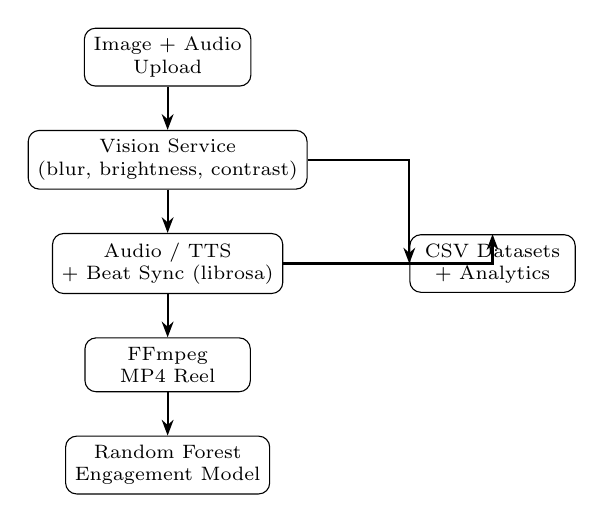
\begin{tikzpicture}[
    node distance=0.55cm and 0.4cm,
    box/.style={draw, rounded corners, align=center, font=\scriptsize, minimum width=2.1cm, minimum height=0.65cm},
    arrow/.style={-{Stealth[length=2mm]}, thick}
]
\node[box] (upload) {Image + Audio\\Upload};
\node[box, below=of upload] (vision) {Vision Service\\(blur, brightness, contrast)};
\node[box, below=of vision] (audio) {Audio / TTS\\+ Beat Sync (librosa)};
\node[box, below=of audio] (ffmpeg) {FFmpeg\\MP4 Reel};
\node[box, right=1.6cm of audio] (data) {CSV Datasets\\+ Analytics};
\node[box, below=of ffmpeg] (ml) {Random Forest\\Engagement Model};

\draw[arrow] (upload) -- (vision);
\draw[arrow] (vision) -- (audio);
\draw[arrow] (audio) -- (ffmpeg);
\draw[arrow] (ffmpeg) -- (ml);
\draw[arrow] (vision.east) -| (data.west);
\draw[arrow] (audio.east) -| (data.north);
\end{tikzpicture}
\caption{High-level DReel AI v2 processing pipeline.}
\label{fig:pipeline}
\end{figure}

\subsection{Audio Beat Synchronization}

Audio is loaded with \texttt{librosa}; onset strength and beat frames yield tempo (BPM) and beat times.
For $N$ images, $N{+}1$ boundary points are sampled from $\{0\} \cup \text{beats} \cup \{T\}$, and durations $d_j = b_{j+1} - b_j$ are clamped to $[0.5, 6.0]$~s and scaled so $\sum d_j = T$.
Features logged per reel: \texttt{tempo\_bpm}, \texttt{beat\_count}, \texttt{avg\_energy}, \texttt{slide\_durations}.

\subsection{Computer Vision Quality Scoring}

Each image is converted to grayscale (downscaled to 800~px max side).
\textbf{Blur} is measured as Laplacian variance $\mathrm{Var}(\nabla^2 I)$---higher values indicate sharper images.
\textbf{Brightness} is mean intensity $\bar{I}$; \textbf{contrast} is pixel standard deviation $\sigma_I$.
The composite score is
\begin{equation}
Q = 0.5\,B_{\mathrm{norm}} + 0.25\,L_{\mathrm{bright}} + 0.25\,C_{\mathrm{norm}},
\end{equation}
where $B_{\mathrm{norm}} = \min(\mathrm{Var}(\nabla^2 I)/500,\,1)$ and $L_{\mathrm{bright}} = \max(0,\,1 - |\bar{I}-128|/128)$.
Images are sorted by descending $Q$ before video assembly.

\subsection{Engagement Prediction}

Eleven features are extracted per reel from audio and vision logs, plus $\mathrm{slide\_std}$ (standard deviation of $\{d_j\}$).
A \textbf{Random Forest Regressor} ($n_{\mathrm{estimators}}{=}120$, $\mathrm{max\_depth}{=}5$) predicts engagement $y \in [1,5]$.
Training labels come from gallery star ratings; unrated reels use a feature-based proxy until sufficient user data is collected.
The model retrains automatically on each new rating.

% ==========================================================
\section{Experiments and Results}
\label{sec:results}

\subsection{Experimental Setup}

\textbf{Environment:} Python~3.11, Flask, \texttt{librosa}~0.11, \texttt{scikit-learn}~1.9, FFmpeg on Windows~11.
\textbf{Datasets:} \texttt{audio\_features.csv} (4 reels), \texttt{image\_features.csv} (7 images), \texttt{engagement\_ratings.csv} (5 user ratings).
\textbf{Metrics:} $R^2$ and MAE for regression; audio--visual gap $|\sum d_j - T|$ for timing comparison.

\subsection{Results}

Table~\ref{tab:audio} summarizes audio features for processed reels.
Beat-sync produces variable slide durations (e.g., 0.94--4.42~s for a 7-image reel at 109.96~BPM), unlike a fixed 1~s schedule.

\begin{table}[t]
\centering
\caption{Audio features for processed reels (sample).}
\label{tab:audio}
\scriptsize
\begin{tabular}{l r r r r}
\toprule
\textbf{Reel ID} & \textbf{Images} & \textbf{Duration (s)} & \textbf{BPM} & \textbf{Avg Slide (s)} \\
\midrule
6f542634 & 10 & 113.5 & 109.96 & 11.35 \\
f08c2cc6 &  7 &  25.1 & 109.96 &  3.59 \\
66432ef0 &  9 &  25.1 & 109.96 &  2.79 \\
ab9bdc64 &  7 &   9.4 & 140.62 &  1.34 \\
\bottomrule
\end{tabular}
\end{table}

Vision scores for reel \texttt{ab9bdc64} ranged from $Q = 0.68$ to $0.96$ (all labeled \emph{good}); the highest-ranked frame had blur variance $1265.7$.

Table~\ref{tab:ml} reports Random Forest performance and top feature importances.

\begin{table}[t]
\centering
\caption{Engagement model results ($n=4$ training reels).}
\label{tab:ml}
\scriptsize
\begin{tabular}{l r}
\toprule
\textbf{Metric / Feature} & \textbf{Value} \\
\midrule
Train $R^2$              & 0.893 \\
Train MAE                & 0.226 \\
Real user ratings        & 3 \\
\midrule
\texttt{slide\_std} (importance)     & 0.347 \\
\texttt{beat\_count}                 & 0.133 \\
\texttt{duration\_sec}               & 0.131 \\
\texttt{image\_count}                & 0.113 \\
\texttt{avg\_slide\_duration}        & 0.097 \\
\bottomrule
\end{tabular}
\end{table}

Beat-sync reduced the mean audio--visual duration gap versus fixed 1~s timing across all four reels (evaluated in Notebook~03).

% ==========================================================
\section{Discussion}
\label{sec:discussion}

The results support the core hypothesis: rhythm-aligned slide timing (\texttt{slide\_std}) is the strongest engagement predictor, suggesting that viewers perceive beat-synced transitions more favourably than uniform pacing.
Computer vision ranking ensures the sharpest frames lead each reel, which is especially useful when users upload images in arbitrary order.

\textbf{Limitations:} (i)~only four reels in the training set---metrics reflect in-sample fit, not generalization; (ii)~beat detection degrades on speech-only or ambient audio; (iii)~quality scoring is rule-based, not deep-learning-based; (iv)~proxy labels for unrated reels introduce label noise.

\textbf{Trade-offs:} Beat-sync adds $\sim$2--3~s processing per reel for librosa analysis, acceptable for offline generation but not real-time streaming.

% ==========================================================
\section{Conclusion and Future Work}
\label{sec:conclusion}

This project delivered DReel AI v2, integrating audio signal processing, computer vision, and machine learning into a functional Flask application with logged datasets, an analytics dashboard, and four Jupyter notebooks.
The pipeline demonstrates a complete data-science workflow from feature engineering to deployed prediction.

Future work includes collecting 50+ user ratings for proper train--test evaluation, CNN-based scene classification for transition selection, deep image-quality models, and Docker-based cloud deployment.

% ==========================================================
\section{Artifacts and Demonstrations}
\label{sec:artifacts}

\begin{itemize}[noitemsep]
    \item \textbf{Source Code:} \url{https://github.com/YOUR-USERNAME/dreel-ai-v2} --- Flask app, services, notebooks, and datasets.
    \item \textbf{Analytics Dashboard:} \texttt{http://localhost:4600/analytics} --- live KPIs and matplotlib charts.
    \item \textbf{Jupyter Notebooks:} \texttt{notebooks/01\_audio\_eda.ipynb} through \texttt{04\_engagement\_model.ipynb}.
    \item \textbf{Video Demo:} \url{https://youtu.be/YOUR-VIDEO-ID} --- end-to-end reel creation and rating workflow.
\end{itemize}

AI-assisted coding tools were used for implementation support; all design decisions, experiments, and reported results reflect the author's own work and understanding.

% ==========================================================
\vfill\pagebreak
{\fontsize{8}{9}\selectfont
\bibliographystyle{IEEEbib}
\begin{thebibliography}{99}

\bibitem{mcfee2015librosa}
B.~McFee \emph{et al.},
``librosa: Audio and music signal analysis in Python,''
in \emph{Proc.\ SciPy}, 2015.

\bibitem{pedregosa2011sklearn}
F.~Pedregosa \emph{et al.},
``Scikit-learn: Machine learning in Python,''
\emph{J.\ Machine Learning Research}, vol.~12, pp.~2825--2830, 2011.

\bibitem{breiman2001rf}
L.~Breiman,
``Random forests,''
\emph{Machine Learning}, vol.~45, no.~1, pp.~5--32, 2001.

\bibitem{pech2000blur}
J.~L.~Pech-Pacheco \emph{et al.},
``Diagnosing of defocus in images by means of blurring measure,''
\emph{Pattern Recognition}, 2000.

\bibitem{ffmpeg}
FFmpeg Project,
\url{https://ffmpeg.org}.

\end{thebibliography}
}

\end{document}
